\documentclass[11pt]{article}
\usepackage[margin=1in]{geometry}
\usepackage[T1]{fontenc}
\usepackage{mathptmx}
\usepackage{courier}
\usepackage{amsmath,amssymb}
\usepackage{graphicx}
\usepackage{booktabs}
\usepackage[numbers,sort&compress]{natbib}
\usepackage{microtype}
\usepackage{xcolor}
\usepackage[hidelinks]{hyperref}
\urlstyle{same}
\usepackage{caption}
\usepackage{enumitem}
\usepackage{multirow}
\usepackage{array}
\usepackage{fancyvrb}
\captionsetup{font=small,labelfont=bf}
\setlist{nosep,leftmargin=1.2em}
\newcommand{\phat}{\hat{P}}
\newcommand{\logit}{\operatorname{logit}}
\newcommand{\sig}[1]{\textbf{#1}}

\title{\textbf{Latent Coherence: Do Frontier Language Models' Probability\\Judgments Obey the Law of Total Probability?}}
\author{Peter Potash\\\small\texttt{pjpotash@gmail.com}}
\date{October 2026}

\begin{document}
\maketitle

\begin{abstract}
A model that reasons by weighing hidden explanations of its evidence, as LawZero's \emph{Scientist AI} proposal envisions, needs probability judgments that fit together. We test whether frontier language models' judgments satisfy the law of total probability, $P(X)=\sum_z P(z)\,P(X\mid z)$, when the latent variable $z$ must be inferred from records in the context. Each item gives a model a short set of records (source track records, an inspection log, a count table, or a fictionalized multi-hop claim from HoVer) and asks, in separate single-turn calls, for $P(X)$, for $P(z)$ over the latent's states, and for $P(X\mid z)$. A causal family applies the same test to $P(y\mid do(x))$ and the back-door adjustment. Every query has an exact ground-truth probability, so coherence and accuracy are measured separately, and a subset of items is asked in three wordings so that incoherence that \emph{persists} across wordings can be separated from rewording noise. Across seven models and 1,590 prompts per model, GPT-6.1 Sol and Claude Opus 5.5 are the most coherent (mean absolute residual 0.08 and 0.12 log-odds). Haiku 5.5, Gemini 3.8 Flash and DeepSeek V4-Pro show substantial persistent incoherence (0.27--0.35 log-odds, with 95\% intervals excluding zero), and they lean in opposite directions, so there is no single shared bias. Reasoning length does not predict coherence: the most coherent models used 400--500 reasoning tokens per answer, while three less coherent ones used 4,400--7,200. Simple consistency checks (normalization, the back-door identity) pass almost everywhere. The failures are specific to reasoning through a latent variable.
\end{abstract}

\section{Introduction}

Many proposals for safer AI systems lean on calibrated probabilistic judgment rather than goal-directed action. LawZero's \emph{Scientist AI} \citep{bengio2025scientist} is a prominent example: a non-agentic system that explains data by positing latent causes and answers queries with probabilities obtained by averaging over those explanations. Averaging over latent explanations is the law of total probability,
\begin{equation}
P(X) \;=\; \sum_z P(z)\,P(X\mid z),
\label{eq:tp}
\end{equation}
and a predictor that violates it gives answers that depend on how a question is decomposed. If such a system is built from, or amortized by, a language model, the model's probability judgments need to obey identities like~\eqref{eq:tp}, at least approximately.

We ask how close current frontier models come. Prior work has shown that language model probability judgments violate simple identities such as complementation and the conjunction rule \citep{zhu2024incoherent}, and that forecasters can be scored by the consistency of logically related forecasts \citep{paleka2025consistency, fluri2023evaluating}. We target a specific and safety-relevant case: coherence under marginalization over a latent variable that the model must \emph{infer from evidence in context}. The latent is never stated. It might be whether a news source is careful, judged from its track record, or which of three faults is present, judged from an inspection log. Reasoning through such a hidden quantity is exactly what Scientist AI asks of its inference machine, and it is where we expect incoherence to concentrate.

\paragraph{Contributions.}
\begin{itemize}
\item An eval of latent coherence with four item families (\S\ref{sec:data}). Three are synthetic, with exact ground truth. The fourth is built from HoVer multi-hop claims \citep{jiang2020hover}, fictionalized so that models cannot answer from memory. A causal family tests $P(y\mid do(x))$ against the back-door adjustment.
\item A noise-corrected decomposition of each model's residual into rewording noise and a \emph{persistent} component (\S\ref{sec:metrics}), so that unstable answers are not mistaken for incoherent judgments.
\item Results for seven frontier models (\S\ref{sec:results}). Two models are coherent to within about 2--3 percentage points. Three have persistent incoherence, leaning in model-specific directions. Reasoning length is not associated with coherence.
\end{itemize}
The code (MIT), data (CC BY-SA 4.0) and evaluation harness are at \href{https://github.com/ppotash/latent-coherence}{github.com/ppotash/latent-coherence}.

\section{Related work}

\paragraph{Coherence of probability judgments.} Human probability judgments are famously incoherent, as in the conjunction fallacy \citep{tversky1983extensional}; \citet{zhu2020bayesian} explain such deviations as the product of sampling-based inference. \citet{zhu2024incoherent} find the same signatures in LLMs, testing identities over events stated directly in the prompt. We test a different identity, marginalization over a latent the model must infer, and we separate wording noise from persistent incoherence instead of pooling them.

\paragraph{Consistency checks.} \citet{fluri2023evaluating} evaluate models on tasks without ground truth by checking logical consistency, and \citet{paleka2025consistency} turn this into arbitrage-based metrics for LLM forecasters. Our items have exact ground truth, which lets us relate incoherence to accuracy directly.

\paragraph{Probabilistic and causal reasoning benchmarks.} QUITE \citep{schrader2024quite} and BLInD \citep{nafar2025reasoning} test Bayesian-network reasoning from text against computed answers. CLadder \citep{jin2023cladder} tests causal queries across Pearl's ladder \citep{pearl2009causality}. These benchmarks score accuracy. We score whether a model's \emph{own} answers agree with each other, which needs no ground truth, and we report accuracy separately. Calibration work \citep{kadavath2022language} asks whether stated confidence matches frequency, a property that is distinct from, and does not imply, coherence across related queries.

\section{The eval}

\subsection{Identities}
\label{sec:identities}

For an item with target event $X$ and latent $Z$ with states $z_1,\dots,z_K$, a model is asked for $\phat(X)$, $\phat(Z=z_k)$ and $\phat(X\mid Z=z_k)$ in $1+2K$ separate single-turn calls, so no answer is ever visible to another query. Its \emph{decomposition} is $D=\sum_k \phat(z_k)\,\phat(X\mid z_k)$. The \textbf{residual} is the gap in log-odds,
\begin{equation}
r \;=\; \logit\phat(X) - \logit D,
\label{eq:resid}
\end{equation}
with probabilities clipped to $[0.01, 0.99]$. Log-odds treat a move from 1\% to 2\% as seriously as one from 33\% to 50\%. Near 50\%, a residual of 0.1 is about 2.5 percentage points. A positive $r$ means the direct answer is higher than the model's decomposition implies.

For causal items the target is $P(y\mid do(x))$: the probability of outcome $y$ if treatment $x$ were \emph{imposed}, rather than merely observed. When $Z$ is the only confounder and is not affected by $X$, the back-door adjustment gives
\begin{equation}
P(y\mid do(x)) \;=\; \sum_z P(z)\,P(y\mid x, z),
\label{eq:backdoor}
\end{equation}
and the residual compares the model's interventional answer with its own adjustment. Normalization ($\sum_k\phat(z_k)=1$ and $\phat(X)+\phat(\lnot X)=1$) is checked separately.

\subsection{Item families}
\label{sec:data}

\begin{table}[t]
\centering\small
\begin{tabular}{@{}l>{\raggedright}p{5.6cm}>{\raggedright\arraybackslash}p{5.4cm}@{}}
\toprule
Family & Records in context & Latent $Z$ \\
\midrule
\texttt{source} & Reports on a claim from 2--4 sources, each with a track record of checked past reports & Whether one source is careful or careless \\
\texttt{diagnostic} & A fault-diagnosis inspection log, with symptom rates for each of three causes & Which of three causes is present \\
\texttt{causal} & A count table over confounder $Z$, treatment $X$ and outcome $Y$ & Back-door adjustment~\eqref{eq:backdoor} \\
\texttt{hover} & A fictionalized HoVer claim split into sub-claims, with reports of the sub-claims from sources of varying reliability & Truth of the bridge sub-claim; a source's kind \\
\bottomrule
\end{tabular}
\caption{Item families. \texttt{source}, \texttt{diagnostic} and \texttt{hover} come in a \emph{full} version, which states every probability, and a \emph{qualitative} version, which gives only verbal descriptions (``usually'', ``most sources are careful''). Appendix~\ref{app:examples} shows complete items.}
\label{tab:families}
\end{table}

Table~\ref{tab:families} summarizes the families. In the \emph{full} versions the item is a well-posed calculation. In the \emph{qualitative} versions the model must form its own numbers. Coherence compares a model with itself, so it is meaningful at both levels. Ground truth always comes from the generating parameters, by exact enumeration for \texttt{source} and \texttt{hover} (validated against rejection sampling), naive Bayes for \texttt{diagnostic}, and empirical frequencies for \texttt{causal}, where the table is the population. Items are filtered so that targets and latent probabilities lie in $[0.1, 0.9]$ and the conditionals differ across latent states by at least 0.10--0.15. Without the filter, coherence would hold trivially near 0 or 1.

The released data contain 1,500 synthetic items (300 per family $\times$ level) and 1,698 HoVer items built from 849 claims. For HoVer, Gemini 3.8 Flash decomposed each claim into logically independent sub-claims and replaced every named entity with an invented name. A second Gemini pass audited the decomposition, and Claude re-verified each accepted claim (Appendix~\ref{app:hover}). The target claim is true exactly when all its sub-claims are, and sub-claim truths and source reliabilities are sampled from stated parameters, so HoVer items also have exact ground truth.

\subsection{Metrics: rewording noise vs persistent incoherence}
\label{sec:metrics}

A nonzero residual has two possible sources. The model's answers may jitter with wording, making $r$ scatter around zero, or its judgments may not fit together, making $r$ stay put however the question is asked. The first is instability; the second is incoherence. To separate them, a subset of \emph{noise-floor} items is asked in three wordings (``What is the probability that\dots'', ``How likely is it that\dots'', ``Estimate the probability that\dots'').

Model each repeated residual as $r_{ik}=\mu_i+e_{ik}$ for instance $i$ (an item $\times$ identity) and wording $k\in\{1,2,3\}$, where $\mu_i$ is the instance's true residual and $e_{ik}$ is wording noise with variance $\sigma^2$. Then
\begin{align}
\widehat{\sigma^2} &= \tfrac{1}{n}\textstyle\sum_i \operatorname{var}_k(r_{ik}) && \text{(rewording noise}=\widehat\sigma), \\
\widehat{\overline{\mu^2}} &= \tfrac{1}{n}\textstyle\sum_i \bar r_i^{\,2} - \widehat{\sigma^2}/3 && \text{(persistent residual}=\textstyle\sqrt{\max(0,\widehat{\overline{\mu^2}})}),
\label{eq:persistent}
\end{align}
where $\bar r_i$ is the mean over wordings. The correction $\widehat{\sigma^2}/3$ removes the noise that remains in a three-wording average. The persistent residual is the root-mean-square size of the instances' true residuals. It satisfies $\overline{\mu^2}=\bar\mu^2+\operatorname{var}(\mu)$, so it counts both a lean shared by all items (the \textbf{direction}, $\bar\mu$) and item-to-item variation. A model that is noisy but coherent scores about 0. 95\% intervals come from 2,000 bootstrap resamples of instances \citep{efron1993bootstrap}.

We also report the \textbf{mean residual}, the average $|r|$ over all items using the first wording only, which reflects noise and persistent incoherence together, and the \textbf{error vs truth}, $|\logit\phat(X)-\logit P(X)|$. Models are compared item by item with a paired sign-flip permutation test on mean $|r|$ (20,000 permutations), Bonferroni-corrected over all 21 model pairs.

\section{Experimental setup}

\paragraph{Sample.} We sampled 20 items from each of the seven (family, level) groups and asked 20 of them in all three wordings. Full-spec synthetic items are solved essentially exactly by every model, so all models except Haiku (which answered everything) were capped at 5 items in each of those three groups. All comparisons use the 95 items answered by every model: 90 with a latent total-probability identity (HoVer items carry two, over the bridge sub-claim and over a source's kind) and 5 causal items with two back-door identities each. Each model answered the same 1,590 prompts.

\paragraph{Models and settings.} Table~\ref{tab:main} lists the models. Each prompt was an independent single-turn call with the system prompt ``Answer the question using only the information provided. Give your final answer as a single probability between 0 and 1.'' The nominal reasoning effort was \emph{medium}. GLM 5.3 and DeepSeek V4-Pro offer no medium setting and ran at \emph{high}. Grok 4.7 ran at \emph{low} because medium was projected to cost about \$94; even so, it reasoned more than every model except DeepSeek. We verified that each provider honors its effort setting by comparing reasoning-token counts across levels on the same prompts. Claude, GPT and Gemini ran through their providers' batch APIs; the others ran synchronously. Responses cut off by the token limit were re-asked with a higher limit (32K for Gemini, 65K for GLM and DeepSeek); none remained truncated. A parser extracts one probability per response, handling both answer-first and answer-last layouts, and was audited by hand on every answer whose reading changed (Appendix~\ref{app:parse}).

\section{Results}
\label{sec:results}

\begin{table}[t]
\centering\footnotesize
\setlength{\tabcolsep}{4.2pt}
\begin{tabular}{@{}lccccccrr@{}}
\toprule
Model & Effort & Mean residual & Persistent & Noise & Dir. & Err.\ vs truth & Tok./ans. & Cost \\
\midrule
GPT-6.1 Sol      & med.  & 0.08 [0.06, 0.11] & \sig{0.08} [0.02, 0.13] & 0.16 & $-0.01$ & 0.34 & 400 & \$4 \\
Claude Opus 5.5  & med.  & 0.12 [0.07, 0.17] & 0.00 [0.00, 0.14] & 0.34 & $+0.01$ & 0.38 & 500 & \$18 \\
DeepSeek V4-Pro  & high  & 0.15 [0.10, 0.21] & \sig{0.27} [0.10, 0.40] & 0.30 & $+0.08$ & 0.37 & 16{,}900 & \$53 \\
Grok 4.7         & low   & 0.21 [0.15, 0.27] & 0.21 [0.00, 0.32] & 0.51 & $+0.05$ & 0.47 & 7{,}200 & \$70 \\
Gemini 3.8 Flash & med.  & 0.26 [0.19, 0.34] & \sig{0.28} [0.10, 0.40] & 0.50 & $-0.11$ & 0.73 & 4{,}400 & \$15 \\
GLM 5.3          & high  & 0.26 [0.20, 0.33] & 0.11 [0.00, 0.25] & 0.53 & $-0.07$ & 0.41 & 6{,}700 & \$54 \\
Claude Haiku 5.5 & med.  & 0.37 [0.27, 0.49] & \sig{0.35} [0.15, 0.48] & 0.64 & $+0.14$ & 0.50 & 1{,}100 & \$1 \\
\bottomrule
\end{tabular}
\caption{Main results on the latent total-probability identity, in log-odds, with 95\% bootstrap CIs. \emph{Mean residual}: average $|r|$ over 90 items (first wording). \emph{Persistent}, \emph{Noise} and \emph{Dir.} (signed mean residual): eq.~\eqref{eq:persistent} on 83 noise-floor instances; bold marks a persistent residual whose CI excludes 0. \emph{Err.\ vs truth}: mean $|\logit\phat(X)-\logit P(X)|$. \emph{Tok./ans.}: mean reasoning tokens per answer. \emph{Cost}: whole run (Haiku 1,890 prompts; DeepSeek at off-peak rates).}
\label{tab:main}
\end{table}

\begin{figure}[t]
\centering
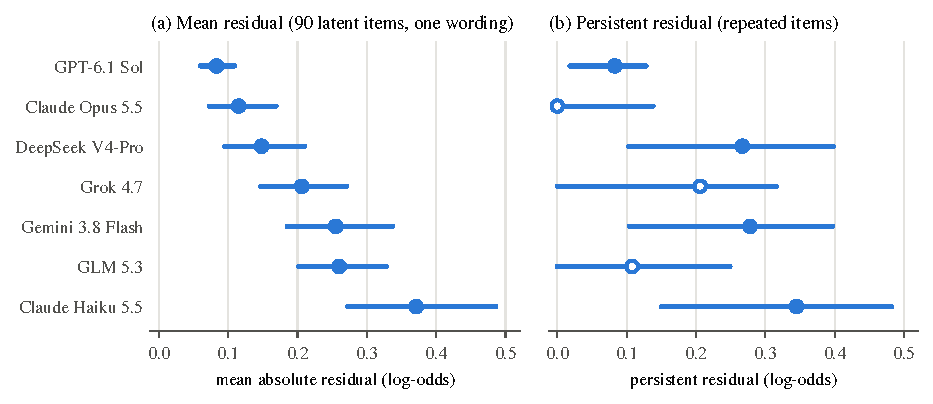
\includegraphics[width=\linewidth]{figures/residuals.pdf}
\caption{(a) Mean absolute residual over all 90 latent items. (b) Persistent residual on the noise-floor items. Bars are 95\% bootstrap CIs; filled markers in (b) have CIs that exclude 0.}
\label{fig:residuals}
\end{figure}

\paragraph{Two tiers, with DeepSeek between them.} Table~\ref{tab:main} and Figure~\ref{fig:residuals} give the main results. GPT-6.1 Sol and Claude Opus 5.5 are the most coherent: their direct answers differ from their own decompositions by 0.08 and 0.12 log-odds on average, about 2--3 percentage points. Their difference is not significant ($p_\text{Bonf}=1.0$). Both are significantly more coherent than Gemini, GLM and Haiku ($p_\text{Bonf}\le 0.008$), and GPT is also more coherent than Grok ($p_\text{Bonf}\le 0.001$). DeepSeek V4-Pro (0.15) cannot be separated statistically from either tier but is significantly more coherent than Haiku. Within the lower tier, only Grok vs Haiku is significant ($p_\text{Bonf}=0.028$). All 21 comparisons are in Appendix~\ref{app:pairwise}.

\paragraph{Noise vs persistent incoherence.} The two residual measures can disagree sharply. GLM and Gemini have the same mean residual (0.26) and similar rewording noise (0.53 and 0.50), but GLM's persistent residual is 0.11 [0, 0.25] while Gemini's is 0.28 [0.10, 0.40]. A single answer from either is equally inconsistent, for different reasons. GLM's residuals scatter around zero as the wording changes, so its incoherence is mostly instability that averaging several samples would reduce. Gemini's residuals hold steady across wordings, so its judgments themselves do not fit together, and re-asking will not fix them. For a system that relies on composing judgments, the persistent kind is the more serious failure. Four models have a persistent residual whose interval excludes 0: Haiku (0.35), Gemini (0.28), DeepSeek (0.27) and, at a small magnitude, GPT (0.08). DeepSeek is distinctive: it has the third-lowest noise (0.30), yet 44\% of its residual variance is persistent, the largest share of any model. It is exact on most items (median residual 0.013) and consistently off on a few.\footnote{The persistent residual is a root-mean-square over noise-floor instances, while the mean residual averages $|r|$ over all items, so a heavy tail can make the former exceed the latter, as for DeepSeek. Each measure should be compared across models rather than against the other.}

\paragraph{No shared direction.} Where incoherence persists, it leans in model-specific directions. Haiku's and DeepSeek's direct answers sit \emph{above} their decompositions ($+0.14$ and $+0.08$ overall, rising to $+0.22$ for Haiku on full HoVer items and $+0.19$ for DeepSeek on qualitative HoVer items). Gemini's sit \emph{below} ($-0.11$ overall, $-0.32$ on qualitative HoVer items). On HoVer items, $X$ is a conjunction of sub-claims, so a positive direction is consistent with overestimating conjunctions relative to their parts. The opposite sign for Gemini shows that this is not a universal property of language models.

\paragraph{Where incoherence appears.} Residuals are near zero on full-spec synthetic items, which are calculations: every model's mean residual there is at most 0.055 (Appendix~\ref{app:groups}). They grow on qualitative items and on HoVer, and peak on qualitative HoVer items, where mean residuals range from 0.16 (GPT) to 0.80 (Haiku). Rewording noise is also higher on qualitative items for six of the seven models. The difficulty is forming numbers from verbal evidence and reasoning through a multi-step latent, not arithmetic.

\begin{figure}[t]
\centering
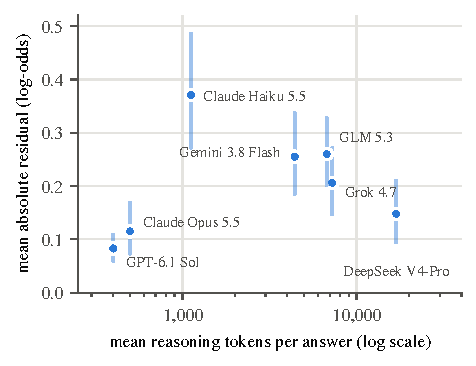
\includegraphics[width=0.56\linewidth]{figures/reasoning.pdf}
\caption{Mean absolute residual (95\% CI) against mean reasoning tokens per answer (log scale).}
\label{fig:reasoning}
\end{figure}

\paragraph{Reasoning length does not predict coherence.} Figure~\ref{fig:reasoning} plots each model's mean residual against its mean reasoning tokens per answer. The two most coherent models reasoned the least (about 400 and 500 tokens). Grok, GLM and Gemini reasoned 9--18 times as much and landed in the lower tier, while DeepSeek reasoned the most (about 16,900 tokens) and placed third. With seven models from six developers and different effort settings, this is an observation rather than a test, and a within-model comparison of effort levels would be the cleaner experiment. It does rule out the simple story that longer reasoning buys coherence.

\paragraph{Simple checks pass; decomposition rarely helps accuracy.} Complementary probabilities sum to 1 for every model (median absolute deviation $\le 0.02$). On causal items, each model's interventional answer matches its own back-door adjustment, with mean residuals at most 0.002 except one item each for GLM and DeepSeek (Appendix~\ref{app:groups}). The failures are therefore specific to marginalizing over an inferred latent. Against ground truth, GPT has the lowest error (0.34) and Gemini the highest (0.73). A model's own decomposition $D$ is rarely more accurate than its direct answer: it is closer to the truth on 39--49\% of items, depending on the model, and it improves the mean error only for Gemini, GPT and Grok, by at most 0.07.

\section{Discussion and limitations}

\paragraph{Implications.} Two frontier models judge probabilities through a latent coherently enough for many purposes, at a level of about 2--3 percentage points. Others carry inconsistencies that persist under rewording, so a system that composes their judgments, as Scientist AI does when it averages over explanations, inherits errors that sampling will not remove. Noise and persistent incoherence call for different remedies, and the persistent residual distinguishes them. The absence of a common direction suggests these failures come from each model's training, not from a shared heuristic, and each model needs to be measured on its own.

\paragraph{Limitations.} Several design choices limit how far the results generalize.
\begin{itemize}
\item \textbf{Settings.} ``Medium'' effort is a vendor label, not a fixed amount of reasoning, and three models deviated from it (Grok low; GLM and DeepSeek high). Temperature is not controllable for most reasoning models, and each prompt was asked once (three times on noise-floor items).
\item \textbf{Sample size.} The noise-floor estimates rest on 83 instances from 20 items, so persistent-residual intervals are wide and per-group breakdowns (Appendix~\ref{app:groups}) are suggestive only.
\item \textbf{Single framing.} We used one conditioning framing (``Suppose you additionally learn, from a completely reliable check\dots''). The harness supports an ``assume'' framing that we did not run.
\item \textbf{Ground truth on qualitative items.} It comes from the hidden generating numbers. Error vs truth there partly measures how a model maps words like ``usually'' to numbers; coherence is unaffected.
\item \textbf{HoVer construction.} Decomposition and fictionalization were done by LLMs, with an LLM audit and an independent cross-check by a model from a second provider; residual decomposition errors would affect ground truth but not coherence.
\item \textbf{Scope.} We test seven API models at one point in time. Decision models that output probabilities directly, and open-weight models run locally, are natural additions.
\end{itemize}

\section{Conclusion}

We introduced an eval of whether language models' probability judgments obey the law of total probability over latent variables inferred from context, with exact ground truth and a decomposition of incoherence into rewording noise and a persistent component. Across seven frontier models, coherence varies by a factor of about 4.5. Persistent incoherence is present in several models and leans in model-specific directions, and it is not explained by how long a model reasons. For proposals that build safe systems from calibrated, composable probability judgments, measuring this kind of coherence directly seems a necessary step.

\bibliographystyle{plainnat}
\bibliography{refs}

\clearpage
\appendix

\section{Example items}
\label{app:examples}

\paragraph{\texttt{source}, full (item \texttt{source-full-00000}).} Context, shown verbatim:
\begin{Verbatim}[fontsize=\scriptsize]
Situation: Some sources have reported on whether the Soustiakloun textile plant
will close by the end of the year.

How sources work: Every source is one of two kinds. A careful source's reports are
correct 85% of the time; a careless source's reports are correct 55% of the time.
Overall, 65% of sources are careful. A source's kind never changes, and different
reports are correct or incorrect independently of one another, given each source's kind.

Base rate: Before any reports, claims of this kind are true 30% of the time.

Track records:
| Source                  | Past reports later checked | Of those, correct |
| Trokeil Staebras        | 0                          | 0                 |
| The Vigoum Gazette      | 3                          | 1                 |
| Braedrouth Triagiabraes | 5                          | 5                 |

Current reports:
- Trokeil Staebras reports that the plant will not close by the end of the year.
- The Vigoum Gazette reports that the plant will not close by the end of the year.
- Braedrouth Triagiabraes reports that the plant will close by the end of the year.
\end{Verbatim}
(In the actual prompt, ``the plant'' is the full name.) Each question is appended and followed by ``Respond with only a probability between 0 and 1.'' Queries and ground truth: $P(X)$ = 0.307 (``What is the probability that the Soustiakloun textile plant will close by the end of the year?''); $P(\text{Gazette careful})$ = 0.258; $P(\text{careless})$ = 0.742; $P(X\mid\text{careful})$ = 0.114 and $P(X\mid\text{careless})$ = 0.374, asked as ``Suppose you additionally learn, from a completely reliable check, the following: The Vigoum Gazette is a careful source. What is the probability that\dots''. Check: $0.258\times 0.114+0.742\times 0.374=0.307$.

\paragraph{\texttt{hover}, qualitative (illustrative item from the gold set).} Original HoVer claim: ``The American publishing company headquartered in Scribner Building publishes the books of the author Donald Richard `Don' DeLillo whose books cover subjects such as the Cold War, mathematics, politics, and economics, and global terrorism.'' Fictionalized sub-claims: (0) ``Ostrander \& Pell is an American publishing company headquartered in the Halvard Building.'' (1, bridge) ``Ostrander \& Pell publishes the books of the author Corwin Ashby.'' (2) ``Corwin Ashby's books cover subjects such as the Cold War, mathematics, politics, economics, and global terrorism.'' The context describes source kinds and base rates only verbally (``A careful source's reports are almost always correct; a careless source's reports are correct only somewhat more often than a coin flip''), lists three sources' track records, and gives five current reports on the sub-claims. The item has two latent identities: over the bridge sub-claim ($P(X)=0.458$; $P(A_1)=0.487$; $P(X\mid A_1)=0.939$; $P(X\mid\lnot A_1)=0$), and over the Baebur Bulletin's kind ($P(\text{careful})=0.791$; $P(X\mid\text{careful})=0.402$; $P(X\mid\text{careless})=0.670$).

\paragraph{\texttt{diagnostic}, qualitative.} ``A maintenance engineer is diagnosing pump unit Paefupeirn. Exactly one of the following faults is present.'' Each of three causes (worn bearing, cracked impeller, clogged intake) is described verbally (``rare as a cause''; ``the outlet pressure is below normal (usually)''), followed by an inspection log of checked findings. Targets: $X$ = failure within 30 days; $Y$ = the result of a test not yet performed. Latent: which fault is present. Both $X$ and $Y$ give a total-probability identity over the three-state latent.

\paragraph{\texttt{causal} (item \texttt{causal-full-00000}).} ``A test lab at Siarethian recorded 500 batteries. Technicians chose the charging protocol for each battery; it was not assigned at random. Assume that the production line is the only factor that affected both the protocol chosen and capacity retention.'' Counts (kept $>$80\% capacity yes/no): older line, slow 22/86; older, fast 20/93; newer, slow 182/51; newer, fast 31/15. The interventional question reads ``A battery is chosen at random from all 500 recorded batteries. Suppose that it is charged with the slow protocol, regardless of whether it came from the older production line. What is the probability that it kept more than 80\% of its capacity after 500 cycles?'' Truth: $P(y\mid do(\text{slow}))=0.442\times0.204+0.558\times0.781=0.526$, while the observational $P(y\mid\text{slow})=0.598$ is inflated because slow charging was used mostly on newer-line batteries.

\section{Dataset construction}
\label{app:hover}

\paragraph{Synthetic families.} \texttt{source}: base rate $\sim U(0.2,0.8)$, share of careful sources $\sim U(0.3,0.7)$, careful accuracy $\in\{0.85,0.90,0.95\}$, careless accuracy $\in\{0.50,0.55,0.60\}$, and per-source track-record lengths from $\{0,2,\dots,12\}$, with all reports sampled from the generative model. \texttt{diagnostic}: cause prior $\sim$ Dirichlet(3,3,3), per-cause symptom and outcome rates, and a sampled inspection log; qualitative items map rates to verbal frequency phrases. \texttt{causal}: population size in $\{200,\dots,600\}$, $P(z)\sim U(0.25,0.75)$, confounded assignment $P(x\mid z)$, and outcome rates $P(y\mid x,z)\sim U(0.05,0.95)$. All families are filtered as described in \S\ref{sec:data}.

\paragraph{HoVer pipeline.} From 1,500 HoVer training claims (500 each of 2, 3 and 4 hops), Gemini 3.8 Flash judged whether each claim is a pure conjunction and, if so, produced 2--5 logically independent, self-contained sub-claims with exact negations, a consistent entity map to invented names, and a bridge index. The instructions require that descriptive modifiers be asserted in exactly one sub-claim, that nothing be dropped, and that comparisons, disjunctions and counting claims be rejected; five hand-written gold decompositions serve as few-shot examples. A second Gemini pass audited each decomposition for conjunction equivalence, independence, exact negations, full fictionalization and self-containment. The 908 accepted claims were re-verified by Claude through the Message Batches API, and the 849 that passed form the released set. 238 HoVer items whose invented names look alike are flagged (\texttt{--exclude-similar-names}). Generation cost about \$45 (Gemini) and \$6 (Claude).

\section{Model settings, cost and parsing}
\label{app:parse}

\begin{table}[h]
\centering\footnotesize
\begin{tabular}{@{}llllrrr@{}}
\toprule
Model & Provider & Effort (levels offered) & Mode & Prompts & Reasoning tok. & Cost (USD) \\
\midrule
Claude Haiku 5.5 & Anthropic & medium & batch & 1{,}890 & 1{,}117 & 0.62 \\
Claude Opus 5.5 & Anthropic & medium & batch & 1{,}590 & 499 & 17.61 \\
GPT-6.1 Sol & OpenAI & medium & batch & 1{,}590 & 400 & 3.96 \\
Gemini 3.8 Flash & Google & medium & batch & 1{,}590 & 4{,}409 & 14.52 \\
Grok 4.7 & xAI & low (low/med./high/xhigh) & sync & 1{,}590 & 7{,}236 & 70.44 \\
GLM 5.3 & Z.ai & high (low/high/max) & sync & 1{,}590 & 6{,}733 & 53.57 \\
DeepSeek V4-Pro (0813) & DeepSeek & high (none/high/max) & sync & 1{,}590 & 16{,}872 & $\approx$53 \\
\bottomrule
\end{tabular}
\caption{Settings and cost. DeepSeek's cost is at off-peak rates (\$106.87 at peak rates). Batch runs are billed at half price.}
\end{table}

\paragraph{Answer parsing.} Most models answer with the number alone or explain and end with it; GLM, and Haiku at times, state the answer first in bold and explain afterwards, and explanations contain other numbers in $[0,1]$. When a response contains several distinct candidates, the parser takes, in order: (1) a last line consisting only of a probability; (2) a first line consisting only of a probability, optionally labelled (``Answer: 0.9''); (3) the number after ``answer is'' or ``final answer''; (4) otherwise the last number. All answers are re-parsed at analysis time so that every model is scored by the same rules. Relative to the values recorded at run time, 125 Haiku answers and 4 GLM answers changed, and every one was checked by hand against its text. No answer from the other five models changed.

\section{Additional results}
\label{app:groups}

\begin{table}[h]
\centering\footnotesize
\setlength{\tabcolsep}{5pt}
\begin{tabular}{@{}lrrrrrrr@{}}
\toprule
Group ($n$ identity instances) & Haiku & Opus & DeepSeek & Gemini & GLM & GPT & Grok \\
\midrule
diagnostic / full (5) & 0.002 & 0.006 & 0.000 & 0.000 & 0.002 & 0.000 & 0.002 \\
source / full (5) & 0.020 & 0.045 & 0.001 & 0.013 & 0.043 & 0.000 & 0.055 \\
diagnostic / qualitative (20) & 0.110 & 0.055 & 0.094 & 0.075 & 0.275 & 0.044 & 0.086 \\
source / qualitative (20) & 0.382 & 0.176 & 0.078 & 0.261 & 0.336 & 0.152 & 0.224 \\
hover / full (40) & 0.376 & 0.046 & 0.186 & 0.169 & 0.109 & 0.012 & 0.234 \\
hover / qualitative (40) & 0.798 & 0.230 & 0.307 & 0.641 & 0.438 & 0.164 & 0.368 \\
\midrule
causal back-door (10) & 0.001 & 0.002 & 0.030 & 0.000 & 0.047 & 0.000 & 0.000 \\
\bottomrule
\end{tabular}
\caption{Mean absolute residual (log-odds) by group, first wording.}
\end{table}

\begin{table}[h]
\centering\footnotesize
\setlength{\tabcolsep}{4.5pt}
\begin{tabular}{@{}lcccc@{}}
\toprule
 & \multicolumn{2}{c}{Full spec (32 instances)} & \multicolumn{2}{c}{Qualitative (51 instances)} \\
\cmidrule(lr){2-3}\cmidrule(l){4-5}
Model & Noise & Persistent & Noise & Persistent \\
\midrule
Claude Haiku 5.5 & 0.37 & 0.34 [0.00, 0.57] & 0.77 & 0.35 [0.00, 0.52] \\
Claude Opus 5.5 & 0.07 & 0.03 [0.00, 0.06] & 0.43 & 0.00 [0.00, 0.17] \\
DeepSeek V4-Pro & 0.28 & \sig{0.36} [0.04, 0.57] & 0.31 & 0.19 [0.00, 0.31] \\
Gemini 3.8 Flash & 0.40 & 0.09 [0.00, 0.20] & 0.56 & \sig{0.35} [0.11, 0.51] \\
GLM 5.3 & 0.45 & 0.00 [0.00, 0.00] & 0.57 & 0.18 [0.00, 0.33] \\
GPT-6.1 Sol & 0.12 & 0.01 [0.00, 0.01] & 0.18 & \sig{0.11} [0.03, 0.16] \\
Grok 4.7 & 0.63 & 0.27 [0.00, 0.46] & 0.41 & 0.15 [0.00, 0.25] \\
\bottomrule
\end{tabular}
\caption{Rewording noise and persistent residual by spec level (noise-floor items). Bold: CI excludes 0.}
\end{table}

\begin{table}[h]
\centering\footnotesize
\begin{tabular}{@{}lccccc@{}}
\toprule
Model & Err.\ direct & Err.\ decomposition & Decomp.\ closer & Normalization (median $|\Sigma-1|$) \\
\midrule
Claude Haiku 5.5 & 0.50 & 0.64 & 44\% & 0.010 \\
Claude Opus 5.5 & 0.38 & 0.42 & 43\% & 0.003 \\
DeepSeek V4-Pro & 0.37 & 0.44 & 40\% & 0.000 \\
Gemini 3.8 Flash & 0.73 & 0.66 & 49\% & 0.010 \\
GLM 5.3 & 0.41 & 0.44 & 39\% & 0.020 \\
GPT-6.1 Sol & 0.34 & 0.33 & 47\% & 0.000 \\
Grok 4.7 & 0.47 & 0.46 & 47\% & 0.000 \\
\bottomrule
\end{tabular}
\caption{Accuracy against ground truth (mean log-odds error over 130 latent-identity instances) for the direct answer and for the model's own decomposition, the share of instances where the decomposition is closer, and normalization.}
\end{table}

\subsection{Pairwise comparisons}
\label{app:pairwise}

\begin{table}[h]
\centering\footnotesize
\setlength{\tabcolsep}{5pt}
\begin{tabular}{@{}llrr@{\hspace{2.2em}}llrr@{}}
\toprule
A & B & $\Delta$ & $p_\text{Bonf}$ & A & B & $\Delta$ & $p_\text{Bonf}$ \\
\midrule
Haiku & Opus & 0.256 & $\le$0.001 & Opus & GPT & $-$0.033 & 1.000 \\
Haiku & DeepSeek & 0.224 & $\le$0.001 & Opus & Grok & $-$0.090 & 0.132 \\
Haiku & Gemini & 0.116 & 0.541 & DeepSeek & Gemini & $-$0.108 & 0.303 \\
Haiku & GLM & 0.112 & 0.819 & DeepSeek & GLM & $-$0.112 & 0.168 \\
Haiku & GPT & 0.289 & $\le$0.001 & DeepSeek & GPT & 0.065 & 0.639 \\
Haiku & Grok & 0.166 & 0.028 & DeepSeek & Grok & $-$0.058 & 1.000 \\
Opus & DeepSeek & $-$0.032 & 1.000 & Gemini & GLM & $-$0.004 & 1.000 \\
Opus & Gemini & $-$0.140 & 0.008 & Gemini & GPT & 0.173 & $\le$0.001 \\
Opus & GLM & $-$0.144 & 0.002 & Gemini & Grok & 0.050 & 1.000 \\
GPT & Grok & $-$0.123 & $\le$0.001 & GLM & GPT & 0.177 & $\le$0.001 \\
 & & & & GLM & Grok & 0.054 & 1.000 \\
\bottomrule
\end{tabular}
\caption{Paired item-level differences $\Delta$ = mean $|r|_A$ $-$ mean $|r|_B$ over 90 latent items, with sign-flip permutation $p$-values (20,000 permutations) Bonferroni-corrected over 21 pairs. ``$\le$0.001'' is the resolution floor of the test after correction.}
\end{table}

\section{Estimator details}

For instance $i$ with wording residuals $r_{i1},r_{i2},r_{i3}$, write $r_{ik}=\mu_i+e_{ik}$ with $\mathbb{E}[e_{ik}]=0$ and $\operatorname{var}(e_{ik})=\sigma^2$. The sample variance across wordings is unbiased for $\sigma^2$, so its average over instances estimates $\sigma^2$. The wording mean $\bar r_i=\mu_i+\bar e_i$ has $\mathbb{E}[\bar r_i^2]=\mu_i^2+\sigma^2/3$, so $\frac1n\sum_i\bar r_i^2-\widehat{\sigma^2}/3$ is unbiased for $\overline{\mu^2}=\frac1n\sum_i\mu_i^2$. Since $\overline{\mu^2}=\bar\mu^2+\frac1n\sum_i(\mu_i-\bar\mu)^2$, the persistent residual combines the shared direction $\bar\mu$ with item-to-item variation; the harness also reports the spread-only quantity (\texttt{systematic\_spread\_sd}), which excludes $\bar\mu$. The square root of a truncated unbiased estimate is biased upward when the true value is near zero, which is why an interval that excludes 0, not the point estimate, is the relevant evidence of persistent incoherence.

\end{document}
